\begin{example}[Задача о встрече]
    Два человека независимо и равномерно выбирают время прихода
    с 12:00 до 13:00. Каждый ждёт другого не более 20 минут.
    Найти вероятность встречи.

    \textbf{Решение.}
    Пусть $x$ и $y$ --- время прихода в минутах после 12:00.
    Тогда
    \[
        \Omega = [0; 60] \times [0; 60].
    \]
    Событие встречи:
    \[
        \mathcal{A}
        = \{(x,y) \in \Omega \colon |x-y| \leq 20\}.
    \]

    \begin{center}
        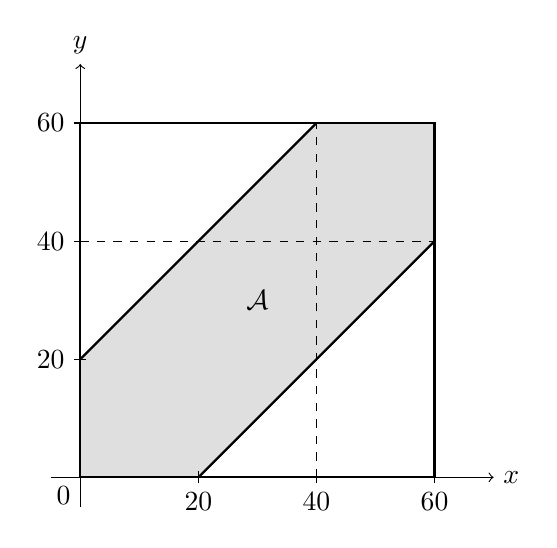
\begin{tikzpicture}[x=0.075cm, y=0.075cm]
            \fill[gray!25]
                (0,0) -- (20,0) -- (60,40) --
                (60,60) -- (40,60) -- (0,20) -- cycle;

            \draw[thick] (0,0) rectangle (60,60);
            \draw[thick] (0,20) -- (40,60);
            \draw[thick] (20,0) -- (60,40);

            \draw[dashed] (0,40) -- (60,40);
            \draw[dashed] (40,0) -- (40,60);

            \draw[->] (-5,0) -- (70,0) node[right] {$x$};
            \draw[->] (0,-5) -- (0,70) node[above] {$y$};

            \node[below left] at (0,0) {$0$};
            \foreach \t in {20,40,60} {
                \draw (\t,1) -- (\t,-1) node[below] {$\t$};
                \draw (1,\t) -- (-1,\t) node[left] {$\t$};
            }

            \node at (30,30) {$\mathcal{A}$};
        \end{tikzpicture}
    \end{center}

    \[
        \Pr(\mathcal{A})
        = \frac{S(\mathcal{A})}{S(\Omega)}
        = \frac{60^2 - 2 \cdot \frac{40^2}{2}}{3600}
        = \frac{2000}{3600}
        = \frac{5}{9}.
    \]
\end{example}

\begin{exercise}[Замечание]
    $\mathcal{F}$ - множество подмножеств $\Omega$, для которых определена $S$ (площадь)
\end{exercise}


\section{Свойства вероятности и основные формулы}
\subsection{$\sigma$ Аддитивность}
\begin{definition}
    Если мы возьмем счетный набор событий $\mathcal{A}_1, \mathcal{A}_2, \dots \mathcal{A}_n\in \mathcal{F}$, (счетное количество событий)\\
    причем дизъюнктивное объединение тоже является событием
    \[
        \mathcal{A} = \bigsqcup_{i=1}^{\infty} \mathcal{A}_i \in \mathcal{F}
    \]
    тогда 
    \[
    \Pr(\mathcal{A})
    =
    \Pr\left(\bigsqcup_{i=1}^{\infty} \mathcal{A}_i\right)
    =
    \Sum{i=1}{\infty} \Pr(\mathcal{A}_i).
    \]
    Это счетная сумма (аддитивность).
\end{definition}

\begin{exercise}[Замечание]
        Обычная аддитивность
        \[
    \Pr\left(\mathcal{A}_1 \sqcup \dots \sqcup \mathcal{A}_n\right)
    =
    \Pr(\mathcal{A}_1) + \dots + \Pr(\mathcal{A}_n).
\]
\end{exercise}

\subsection{Условная вероятность}
\begin{definition}
    Пусть $\mathcal{A}, \mathcal{B} \in \mathcal{F}$
    и $\Pr(\mathcal{B}) \neq 0$.
    Условной вероятностью события $\mathcal{A}$
    при условии события $\mathcal{B}$ называется число
    \[
        \Pr(\mathcal{A} \mid \mathcal{B})
        =
        \frac{\Pr(\mathcal{A} \cap \mathcal{B})}{\Pr(\mathcal{B})}.
    \]
\end{definition}

\begin{Proof}[Обоснование в классической модели.]

Пусть $\Pr(\mathcal{B}) > 0$. Если известно, что событие
$\mathcal{B}$ произошло, то остаются только исходы из
$\mathcal{B}$, которые по-прежнему равновероятны.
Из них событию $\mathcal{A}$ благоприятствуют исходы
из $\mathcal{A} \cap \mathcal{B}$. Поэтому
\[
    \Pr(\mathcal{A} \mid \mathcal{B})
    =
    \frac{|\mathcal{A} \cap \mathcal{B}|}{|\mathcal{B}|}
    =
    \frac{
        |\mathcal{A} \cap \mathcal{B}| / |\Omega|
    }{
        |\mathcal{B}| / |\Omega|
    }
    =
    \frac{\Pr(\mathcal{A} \cap \mathcal{B})}{\Pr(\mathcal{B})}.
\]
\end{Proof}

\begin{center}
    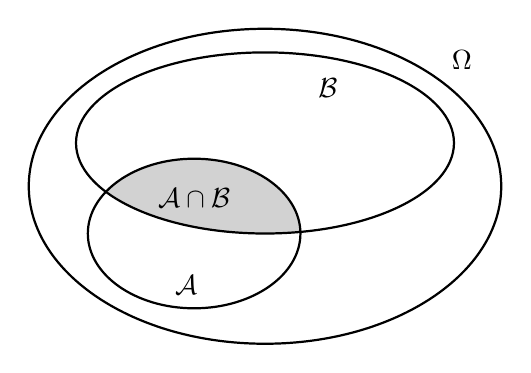
\begin{tikzpicture}[scale=1]
        % Пространство элементарных исходов.
        \draw[thick] (0,0) ellipse (3cm and 2cm);
        \node at (2.5,1.6) {$\Omega$};

        % Пересечение событий.
        \begin{scope}
            \clip (-0.9,-0.6) ellipse (1.35cm and 0.95cm);
            \fill[gray!35] (0,0.55) ellipse (2.4cm and 1.15cm);
        \end{scope}

        % События.
        \draw[thick]
            (-0.9,-0.6) ellipse (1.35cm and 0.95cm);
        \draw[thick]
            (0,0.55) ellipse (2.4cm and 1.15cm);

        \node at (-1,-1.25) {$\mathcal{A}$};
        \node at (0.8,1.25) {$\mathcal{B}$};
        \node at (-0.9,-0.15) {$\mathcal{A}\cap\mathcal{B}$};
    \end{tikzpicture}
\end{center}

\begin{example}[Пример: Условная вероятность при броске двух костей]
    Бросаются две игральные кости
    Обозначим через $\Sigma$ сумму выпавших очков

    Если $\Sigma = 6$, возможны исходы
    \[
        \{(1,5),(2,4),(3,3),(4,2),(5,1)\}.
    \]

    
    \[
        \Pr(\text{есть двойка} \mid \Sigma = 6)
        =
        \frac{
            \Pr\left(\{(2,4),(4,2)\}\right)
        }{
            \Pr\left(\{(1,5),(2,4),(3,3),(4,2),(5,1)\}\right)
        }
        =
        \frac{2/36}{5/36}
        =
        \frac{2}{5}.
    \]

    Если $\Sigma = 4$, возможны исходы
    \[
        \{(1,3),(2,2),(3,1)\}.
    \]
    
    
    \[
        \Pr(\text{есть двойка} \mid \Sigma = 4)
        =
        \frac{
            \Pr\left(\{(2,2)\}\right)
        }{
            \Pr\left(\{(1,3),(2,2),(3,1)\}\right)
        }
        =
        \frac{1/36}{3/36}
        =
        \frac{1}{3}.
    \]
\end{example}

\subsection{Формула полной вероятности}
\begin{definition}
    Пусть $\mathcal{A}_1, \mathcal{A}_2, \dots \mathcal{A}_n\in \mathcal{F}$, причем
    \[
        \Pr(\mathcal{A}_k) \neq 0, \qquad
        \
        \qquad
        \bigsqcup_{k=1}^{\infty} \mathcal{A}_k = \Omega.
    \]
    Тогда
    \[
        \Pr(\mathcal{B})
        =
        \sum_{k=1}^{\infty}
        \Pr(\mathcal{B} \mid \mathcal{A}_k) \cdot
        \Pr(\mathcal{A}_k).
    \]
\end{definition}
\begin{example}[Пример]
    Есть две урны:
    \begin{itemize}
        \item в первой --- 3 красных и 2 чёрных шара;
        \item во второй --- 1 красный и 4 чёрных шара.
    \end{itemize}
    Сначала равновероятно выбирают одну из урн, затем
    случайно вытаскивают из неё один шар.
    Найти вероятность того, что шар красный.
\end{example}

\begin{solution}
    Обозначим события:
    \[
        \mathcal{A}_1 = \{\text{выбрана первая урна}\},
        \qquad
        \mathcal{A}_2 = \{\text{выбрана вторая урна}\},
    \]
    \[
        \mathcal{B} = \{\text{вытащен красный шар}\}.
    \]
    События $\mathcal{A}_1$ и $\mathcal{A}_2$ несовместны
    и образуют полную группу:
    \[
        \mathcal{A}_1 \sqcup \mathcal{A}_2 = \Omega,
        \qquad
        \Pr(\mathcal{A}_1) = \Pr(\mathcal{A}_2) = \frac{1}{2}.
    \]
    Условные вероятности вытащить красный шар:
    \[
        \Pr(\mathcal{B} \mid \mathcal{A}_1) = \frac{3}{5},
        \qquad
        \Pr(\mathcal{B} \mid \mathcal{A}_2) = \frac{1}{5}.
    \]
    По формуле полной вероятности:
    \[
        \begin{aligned}
            \Pr(\mathcal{B})
            &=
            \Pr(\mathcal{B} \mid \mathcal{A}_1)
            \cdot \Pr(\mathcal{A}_1)
            +
            \Pr(\mathcal{B} \mid \mathcal{A}_2)
            \cdot \Pr(\mathcal{A}_2)
            \\
            &=
            \frac{3}{5} \cdot \frac{1}{2}
            +
            \frac{1}{5} \cdot \frac{1}{2}
            =
            \frac{2}{5}.
        \end{aligned}
    \]
\end{solution}


\subsection{Формула умножения вероятности}
\begin{definition}
    3 красных, 4 черных шариков, вытаскиваем последовательно
    \[
        \Pr(\text{черный -> черный -> красный}) = \frac{4}{7} \cdot \frac{3}{6} \cdot \frac{3}{5}
    \]

\end{definition}

\begin{Proof}
    Пусть $\Pr(\mathcal{A}_1 \cap \dots \cap \mathcal{A}_{n-1}) > 0$.
    По определению условной вероятности:
    \[
        \Pr(B \mid A)
        =
        \frac{\Pr(A \cap B)}{\Pr(A)}
        \implies
        \Pr(A \cap B) = \Pr(A)\Pr(B \mid A).
    \]
    Последовательно применяя эту формулу, получаем
    \[
        \begin{aligned}
            &\Pr(\mathcal{A}_1 \cap \dots \cap \mathcal{A}_n)
            \\
            &=
            \Pr(\mathcal{A}_1 \cap \dots \cap \mathcal{A}_{n-1})
            \Pr(\mathcal{A}_n \mid
                \mathcal{A}_1 \cap \dots \cap \mathcal{A}_{n-1})
            \\
            &= \dots =
            \Pr(\mathcal{A}_1)
            \Pr(\mathcal{A}_2 \mid \mathcal{A}_1)
            \cdot \ldots \cdot
            \Pr(\mathcal{A}_n \mid
                \mathcal{A}_1 \cap \dots \cap \mathcal{A}_{n-1}).
        \end{aligned}
    \]
    При подстановке условных вероятностей дробями
    множители последовательно сокращаются:
    \[
        \begin{aligned}
            &\Pr(\mathcal{A}_1)
            \cdot
            \frac{\Pr(\mathcal{A}_1 \cap \mathcal{A}_2)}
                 {\Pr(\mathcal{A}_1)}
            \cdot \ldots \cdot
            \frac{\Pr(\mathcal{A}_1 \cap \dots \cap \mathcal{A}_n)}
                 {\Pr(\mathcal{A}_1 \cap \dots \cap \mathcal{A}_{n-1})}
            \\
            &= \Pr(\mathcal{A}_1 \cap \dots \cap \mathcal{A}_n).
        \end{aligned}
    \]
\end{Proof}
\subsection{Формула Байеса}

\begin{theorem}[Формула Байеса]
    Пусть события $\mathcal{B}_1,\mathcal{B}_2,\dots$
    :
    \[
        \bigsqcup_{i=1}^{\infty} \mathcal{B}_i = \Omega,
        \qquad
        \Pr(\mathcal{B}_i) \neq 0.
    \]
    Тогда для события $\mathcal{A}$, такого что
    $\Pr(\mathcal{A}) \neq 0$, выполняется
    \[
        \Pr(\mathcal{B}_k \mid \mathcal{A})
        =
        \frac{\Pr(\mathcal{A} \cap \mathcal{B}_k)}
             {\Pr(\mathcal{A})}
        =
        \frac{
            \Pr(\mathcal{A} \mid \mathcal{B}_k)
            \cdot \Pr(\mathcal{B}_k)
        }{
            \Sum{i=1}{\infty}
            \Pr(\mathcal{A} \mid \mathcal{B}_i)
            \cdot \Pr(\mathcal{B}_i)
        }.
    \]
    Для конечной полной группы из $n$ событий
    $\Sigma$ берётся от $1$ до $n$.
\end{theorem}

\subsection{Независимость событий}

\begin{definition}
    События $\mathcal{A}, \mathcal{B} \in \mathcal{F}$
    называются \textbf{независимыми}, если
    \[
        \Pr(\mathcal{A} \cap \mathcal{B})
        =
        \Pr(\mathcal{A}) \cdot \Pr(\mathcal{B}).
    \]
    Обозначение:
    \[
        \mathcal{A} \perp\!\!\!\perp \mathcal{B}.
    \]
    Если $\Pr(\mathcal{B}) > 0$, это равносильно условию
    \[
        \Pr(\mathcal{A} \mid \mathcal{B})
        =
        \frac{\Pr(\mathcal{A} \cap \mathcal{B})}{\Pr(\mathcal{B})}
        =
        \Pr(\mathcal{A}).
    \]
    То есть наступление события $\mathcal{B}$ не меняет
    вероятность события $\mathcal{A}$.
\end{definition}

\subsubsection{Попарная независимость и независимость в совокупности}

\begin{definition}[Попарная независимость]
    События $\mathcal{A}_1,\dots,\mathcal{A}_n$
    называются \textbf{попарно независимыми}, если
    \[
        \Pr(\mathcal{A}_i \cap \mathcal{A}_j)
        =
        \Pr(\mathcal{A}_i)\cdot\Pr(\mathcal{A}_j)
        \qquad
        \forall\,1 \leq i < j \leq n.
    \]
\end{definition}





\begin{definition}[Независимость в совокупности]
    События $\mathcal{A}_1,\dots,\mathcal{A}_n$
    называются \textbf{независимыми в совокупности}, если
    для любого $k \in \{2,\dots,n\}$ и любых индексов
    \[
        1 \leq i_1 < i_2 < \dots < i_k \leq n
    \]
    выполняется
    \[
        \Pr(\mathcal{A}_{i_1} \cap \dots \cap \mathcal{A}_{i_k})
        =
        \Pr(\mathcal{A}_{i_1})\cdot\ldots\cdot
        \Pr(\mathcal{A}_{i_k}).
    \]
    То есть равенство проверяется для любой выбранной группы
    событий, а не только для пар.
\end{definition}

\begin{exercise}[Замечание]
    Из независимости в совокупности следует попарная независимость.
    Обратное утверждение в общем случае неверно.
\end{exercise}

\begin{example}[Пример Бернштейна]
    Равновероятно выбирается одна из четырёх вершин тетраэдра
    \begin{center}
        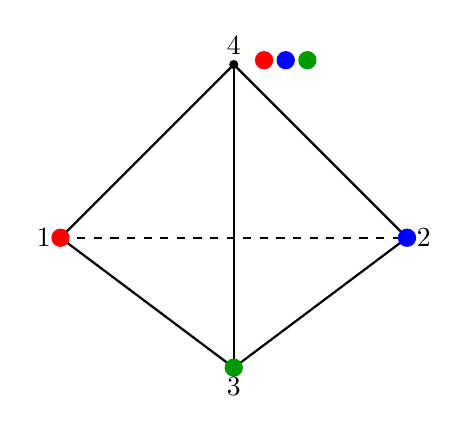
\begin{tikzpicture}[scale=1.1]
            \coordinate (v1) at (-2,0);
            \coordinate (v2) at (2,0);
            \coordinate (v3) at (0,-1.5);
            \coordinate (v4) at (0,2);

            \draw[thick] (v1) -- (v4) -- (v2) -- (v3) -- cycle;
            \draw[thick] (v4) -- (v3);
            \draw[thick,dashed] (v1) -- (v2);

            \fill[red] (v1) circle (3pt);
            \fill[blue] (v2) circle (3pt);
            \fill[green!60!black] (v3) circle (3pt);
            \fill (v4) circle (1.5pt);

            \node[left] at (v1) {$1$};
            \node[right] at (v2) {$2$};
            \node[below] at (v3) {$3$};
            \node[above] at (v4) {$4$};

            \fill[red] (0.35,2.05) circle (3pt);
            \fill[blue] (0.60,2.05) circle (3pt);
            \fill[green!60!black] (0.85,2.05) circle (3pt);
        \end{tikzpicture}
    \end{center}

    Получаем классическую модель:
    \[
        \Omega = \{\omega_1,\omega_2,\omega_3,\omega_4\},
        \qquad
        \Pr(\{\omega_i\}) = \frac14.
    \]
    Рассмотрим события:
    \[
        \begin{aligned}
            \mathcal{A}_1
            &= \{\text{выбранная вершина имеет красную отметку}\}
            = \{\omega_1,\omega_4\},\\
            \mathcal{A}_2
            &= \{\text{выбранная вершина имеет синюю отметку}\}
            = \{\omega_2,\omega_4\},\\
            \mathcal{A}_3
            &= \{\text{выбранная вершина имеет зелёную отметку}\}
            = \{\omega_3,\omega_4\}.
        \end{aligned}
    \]
    Каждое событие содержит два исхода, поэтому
    \[
        \Pr(\mathcal{A}_1)
        =
        \Pr(\mathcal{A}_2)
        =
        \Pr(\mathcal{A}_3)
        =
        \frac12.
    \]

    \[
        \Pr(\mathcal{A}_i \cap \mathcal{A}_j)
        =
        \frac14
        =
        \frac12 \cdot \frac12
        =
        \Pr(\mathcal{A}_i)\Pr(\mathcal{A}_j),
        \qquad i \neq j.
    \]
    Следовательно, события попарно независимы.

    \[
        \Pr(\mathcal{A}_1 \cap \mathcal{A}_2 \cap \mathcal{A}_3)
        =
        \frac14
        \neq
        \frac18
        =
        \Pr(\mathcal{A}_1)\Pr(\mathcal{A}_2)\Pr(\mathcal{A}_3).
    \]
    Независимости в совокупности нет.
\end{example}




\begin{example}[Пример: Формула умножения и независимость событий. Как их правильно отличать?]
    В урне 3 красных и 4 чёрных шара. Последовательно
    вытаскивают два шара. Обозначим события
    \[
        \mathcal{A} = \{\text{первый шар чёрный}\},
        \qquad
        \mathcal{B} = \{\text{второй шар чёрный}\}.
    \]

    \textbf{1. Без возвращения.}

    Если первый шар оказался чёрным, в урне осталось
    3 чёрных шара из 6. Поэтому
    \[
        \Pr(\mathcal{B} \mid \mathcal{A}) = \frac{3}{6}.
    \]
    По формуле полной вероятности
    \[
        \Pr(\mathcal{B})
        =
        \frac{4}{7} \cdot \frac{3}{6}
        +
        \frac{3}{7} \cdot \frac{4}{6}
        =
        \frac{4}{7}.
    \]
    Следовательно,
    \[
        \Pr(\mathcal{B} \mid \mathcal{A})
        \neq
        \Pr(\mathcal{B}),
    \]
    то есть события зависимы. По формуле умножения:
    \[
        \Pr(\mathcal{A} \cap \mathcal{B})
        =
        \Pr(\mathcal{A})
        \cdot \Pr(\mathcal{B} \mid \mathcal{A})
        =
        \frac{4}{7} \cdot \frac{3}{6}
        =
        \frac{2}{7}.
    \]

    \textbf{2. С возвращением и перемешиванием.}

    Первый шар возвращают в урну и перемешивают её содержимое.
    Перед вторым вытаскиванием состав урны прежний,
    поэтому события независимы:
    \[
        \Pr(\mathcal{B} \mid \mathcal{A})
        =
        \Pr(\mathcal{B})
        =
        \frac{4}{7}.
    \]
    Формула умножения принимает вид
    \[
        \Pr(\mathcal{A} \cap \mathcal{B})
        =
        \Pr(\mathcal{A}) \cdot \Pr(\mathcal{B})
        =
        \frac{4}{7} \cdot \frac{4}{7}
        =
        \frac{16}{49}.
    \]

    Формула умножения применима в обоих случаях.
    Независимость позволяет заменить условную вероятность
    $\Pr(\mathcal{B} \mid \mathcal{A})$ на $\Pr(\mathcal{B})$.
\end{example}

\section{Системы множеств}

\subsection{Полукольцо}
\begin{definition}
    Система множеств $S$ называется полукольцом, если
    \begin{enumerate}[label=\arabic*)]
        \item $\varnothing \in S$
        \item $A, B \in S,\text{ то }  A \cap B \in S $ - Замкнутость относительно операции пересечения
        \item $A, B \in S \text{, то  } \exists A_1, ..., A_n \in S:$
        \\
        A $\setminus$ B = $\bigsqcup_{i=1}^{n} \mathcal{A}_i$
        
        
    \end{enumerate}
\end{definition}
\begin{example}
    Промежутки на $\mathbb{R}$
    Рассмотрим систему $S$ всех промежутков на $\mathbb{R}$, \\
    Проверим свойства полукольца

    \begin{enumerate}[label=\arabic*)]
        \item $S \neq \varnothing$, поскольку, например, $[0;8] \in S$.

        \item Пересечение двух промежутков является промежутком
        либо пустым множеством. Следовательно,
        \[
            A, B \in S \implies A \cap B \in S.
        \]

        \item Разность двух промежутков представляется
        как объединение не более двух непересекающихся
        промежутков.

        Например, пусть
        \[
            A = [0;8], \qquad B = [1;3).
        \]
        Тогда
        \[
            A \setminus B = [0;1) \sqcup [3;8]
        \]
        

        Обозначив
        \[
            A_1 = [0;1), \qquad A_2 = [3;8],
        \]
        получаем
        \[
            A \setminus B = A_1 \sqcup A_2,
            \qquad A_1, A_2 \in S,
            \qquad A_1 \cap A_2 = \varnothing.
        \]
    \end{enumerate}

    Таким образом, система $S$ является полукольцом
\end{example}

\subsubsection{Симметрическая разность}

\begin{definition}
    Симметрической разностью множеств $A$ и $B$
    называется множество элементов, принадлежащих
    ровно одному из этих множеств:
    \[
        A \triangle B
        =
        (A \cup B) \setminus (A \cap B)
        =
        (A \setminus B) \sqcup (B \setminus A).
    \]
\end{definition}

% В преамбулу: \usepackage{tikz}
\begin{center}
    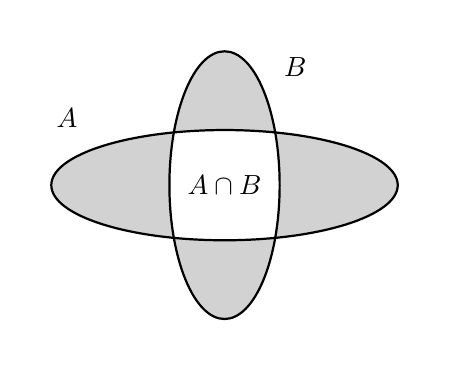
\begin{tikzpicture}
        \begin{scope}
            \clip (-2.5,-2) rectangle (2.5,2);
            \fill[gray!35, even odd rule]
                (0,0) ellipse (2.2cm and 0.7cm)
                (0,0) ellipse (0.7cm and 1.7cm);
        \end{scope}

        \draw[thick] (0,0) ellipse (2.2cm and 0.7cm);
        \draw[thick] (0,0) ellipse (0.7cm and 1.7cm);

        \node at (-2,0.85) {$A$};
        \node at (0.9,1.5) {$B$};
        \node at (0,0) {$A \cap B$};
    \end{tikzpicture}
\end{center}
\subsection{Кольцо}
\begin{definition}
    Система множеств $R$ называется \textbf{кольцом}, если
    \begin{enumerate}[label=\arabic*)]
        \item $\varnothing \neq R$;
        \item $\forall$ $A, B \in R$ выполняется
        \[
            A \cap B \in R,
            \qquad
            A \triangle B \in R.
        \]
    \end{enumerate}
\end{definition}
\begin{exercise}[Замечание]
        Кольцо замкнуто относительно всех операций
    \[
        A, B \in R
        \implies
        A \cup B \in R,
        \qquad
        A \setminus B \in R
    \]
    
    \begin{center}
        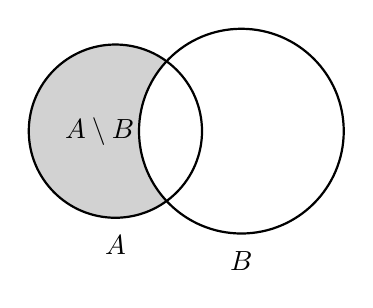
\begin{tikzpicture}
    
            \begin{scope}
                \clip (-0.8,0) circle (1.1cm);
                \fill[gray!35, even odd rule]
                    (-3,-2) rectangle (3,2)
                    (0.8,0) circle (1.3cm);
            \end{scope}

            \draw[thick] (-0.8,0) circle (1.1cm);
            \draw[thick] (0.8,0) circle (1.3cm);

            \node at (-0.8,-1.45) {$A$};
            \node at (0.8,-1.65) {$B$};
            \node at (-1,0) {$A \setminus B$};
        \end{tikzpicture}
    \end{center}
\end{exercise}

\begin{exercise}[Замечание]
    Любое кольцо является полукольцом.
    Проверим условия:
    \begin{enumerate}[label=\arabic*)]
        \item $\varnothing \in R$, поэтому $R \neq \varnothing$.

        \item Если $A, B \in R$, то $A \cap B \in R$ - верно

        \item Если $A, B \in R$, то $A \setminus B \in R$.
        Поэтому достаточно взять $A_1 = A \setminus B$:
        \[
            A \setminus B = \bigsqcup_{i=1}^{1} A_i,
            \qquad A_1 \in R.
        \]
    \end{enumerate}
\end{exercise}

\begin{exercise}[Замечание]
    Пусть $S = \{A_\alpha\}_{\alpha \in I}$ --- полукольцо.
    Положим
    \[
        \Omega = \bigcup_{\alpha \in I} A_\alpha.
    \]
    Тогда
    \[
        S \subset 2^\Omega.
    \]
    В частности, существует кольцо $R$, содержащее $S$:
    можно взять $R = 2^\Omega$
    \[
        S \subset R = 2^\Omega.
    \]
    Вывод: если есть полукольцо, всегда есть кольцо, которое содержит данное полукольцо
\end{exercise}

\subsection{Наименьшее кольцо}
\begin{definition}
    Пусть $\chi$ --- система множеств.
    Кольцо $R(\chi)$ называется \textbf{наименьшим кольцом,
    содержащим $\chi$}, если
    \begin{enumerate}[label=\arabic*)]
        \item $\chi \subset R(\chi)$;
        \item $\forall$ $R_1$, кольца: если $\chi$ $\subset$ $R_1$, то верно
        \[
            R(\chi) \subset R_1.
        \]
    \end{enumerate}

\end{definition}

\subsubsection{Существование наименьшего кольца}

\begin{theorem}
    Для любой системы множеств $\chi$ существует
    наименьшее кольцо $R(\chi)$, содержащее $\chi$
\end{theorem}

\begin{Proof}
    \begin{enumerate}[label=\arabic*)]
        \item Хотя бы одно кольцо, содержащее $\chi$, существует:
        \[
            \Omega = \bigcup_{A_i \in \chi} A_i,
            \qquad R_1 = 2^\Omega
        \]

        \item Рассмотрим все кольца подмножеств $\Omega$,
        содержащие $\chi$, и обозначим их
        $\{R_\alpha\}_{\alpha \in I}$. Положим
        \[
            R_0 = \bigcap_{\alpha \in I} R_\alpha
        \]
        Докажем, что $R_0 = R(\chi)$
    \end{enumerate}

    \textbf{I. $R_0$ --- кольцо.}
    \begin{enumerate}[label=\arabic*)]
        \item Поскольку $\varnothing \in R_\alpha$
        для каждого $\alpha \in I$, имеем
        \[
            \varnothing \in
            \bigcap_{\alpha \in I} R_\alpha = R_0.
        \]

        \item Пусть $A, B \in R_0$. Тогда
        \[
            A, B \in R_\alpha
            \qquad \forall \alpha \in I.
        \]
        Каждая система $R_\alpha$ является кольцом, поэтому
        \[
            A \cap B \in R_\alpha,
            \qquad
            A \triangle B \in R_\alpha
            \qquad \forall \alpha \in I.
        \]
        Следовательно,
        \[
            A \cap B \in R_0,
            \qquad
            A \triangle B \in R_0.
        \]
    \end{enumerate}

    \textbf{II. $\chi$  $\subset$ $R_0$}

    Поскольку $\chi \subset R_\alpha$ для каждого $\alpha \in I$,
    \[
        \chi \subset \bigcap_{\alpha \in I} R_\alpha = R_0.
    \]

    \textbf{III. $R_0$ --- наименьшее такое кольцо.}

Пусть $R'$ --- произвольное кольцо, содержащее $\chi$:
\[
    \chi \subset R'.
\]
Тогда $R'$ входит в систему $\{R_\alpha\}_{\alpha \in I}$,
то есть
\[
    \exists \alpha_0 \in I \colon R' = R_{\alpha_0}
\]
Следовательно,
\[
    R_0 = \bigcap_{\alpha \in I} R_\alpha
    \subset R_{\alpha_0} = R'.
\]
\end{Proof}

\subsection{Наименьшее кольцо, содержащее полукольцо}
\begin{theorem}
    Пусть $S$ --- полукольцо. Тогда
    \[
        R(S)
        =
        \left\{
            \bigsqcup_{i=1}^{n} A_i
            \;\middle|\;
            n \in \mathbb{N},\;
            A_i \in S\;
        \right\}.
    \]
\end{theorem}
\begin{Proof}
    Обозначим множество из правой части как $K = \left\{ \bigsqcup_{i=1}^{n} A_i \;\middle|\; A_i \in S \right\}$. 
    Нам нужно доказать два включения: $K \subset R(S)$ и $R(S) \subset K$. %[cite: 9]

    \textbf{1. Включение $K \subset R(S)$.} \\
    Возьмем произвольный элемент $x \in K$. По определению множества $K$, $x$ представим в виде дизъюнктного объединения конечного числа элементов полукольца:
    \[
        x = \bigsqcup_{i=1}^{n} A_i, \quad A_i \in S.
    \]
    Поскольку $S \subset R(S)$ (по определению наименьшего кольца), каждый $A_i \in R(S)$. Так как $R(S)$ --- кольцо, оно замкнуто относительно конечных объединений, следовательно, $x \in R(S)$. Включение доказано. %[cite: 9]

    \textbf{2. Включение $R(S) \subset K$.} \\
    Чтобы доказать это включение, достаточно показать, что $K$ само является кольцом. Так как $K$ содержит $S$ (достаточно взять $n=1$), а $R(S)$ --- \textit{наименьшее} кольцо, содержащее $S$, из того, что $K$ --- кольцо, мгновенно последует $R(S) \subset K$. %[cite: 9]
    
    Для доказательства того, что $K$ --- кольцо, нам понадобится вспомогательная лемма.
\end{Proof}

\subsection{Лемма о разности элементов полукольца}

\begin{lemma}
    Если $A, B_1, B_2, \dots, B_m \in S$, то существуют такие $A_1, A_2, \dots, A_n \in S$, что:
    \[
        A \setminus B_1 \setminus B_2 \setminus \dots \setminus B_m = \bigsqcup_{i=1}^{n} A_i.
    \]
\end{lemma}

\begin{Proof}[Доказательство леммы]
    Доказывать будем по индукции по $m$. %[cite: 9]
    
    \textbf{База индукции ($m=1$):} \\
    Утверждение $A \setminus B_1 = \bigsqcup_{i=1}^{n} A_i$ выполняется по определению полукольца (свойство разности). %[cite: 9]

    \textbf{Шаг индукции:} \\
    Пусть утверждение верно для $m$. Докажем для $m+1$. %[cite: 9]
    \[
        A \setminus B_1 \setminus \dots \setminus B_m \setminus B_{m+1} = \left( \bigsqcup_{i=1}^{n} A_i \right) \setminus B_{m+1} = \bigsqcup_{i=1}^{n} (A_i \setminus B_{m+1}).
    \]
    Так как $A_i \in S$ и $B_{m+1} \in S$, по определению полукольца разность $A_i \setminus B_{m+1}$ представима в виде $\bigsqcup_{j=1}^{k_i} C_{ij}$, где $C_{ij} \in S$. %[cite: 9]
    Тогда:
    \[
        \bigsqcup_{i=1}^{n} (A_i \setminus B_{m+1}) = \bigsqcup_{i=1}^{n} \left( \bigsqcup_{j=1}^{k_i} C_{ij} \right) = \bigsqcup_{i, j} C_{ij}.
    \]
    Получили дизъюнктивное объединение конечного числа элементов из $S$. Лемма доказана. %[cite: 9]
\end{Proof}

\begin{Proof}[{{Продолжение доказательства теоремы (проверка, что $K$ --- кольцо)}}]
    \begin{enumerate}[label=\arabic*)]
        \item $\varnothing \in K$, так как $S \subset K$ и $\varnothing \in S$. %[cite: 10]
        \item Пусть $P, Q \in K$. Докажем, что $P \cap Q \in K$ и $P \triangle Q \in K$. %[cite: 10]
        
        По определению $K$, элементы $P$ и $Q$ имеют вид:
        \[
            P = \bigsqcup_{i=1}^{n} P_i, \quad Q = \bigsqcup_{j=1}^{m} Q_j, \qquad P_i, Q_j \in S.
        \]
        
        \textbf{Пересечение:}
        \[
            P \cap Q = \left( \bigsqcup_{i=1}^{n} P_i \right) \cap \left( \bigsqcup_{j=1}^{m} Q_j \right) = \bigsqcup_{i=1}^{n} \bigsqcup_{j=1}^{m} (P_i \cap Q_j).
        \]
        Обозначим $D_{ij} = P_i \cap Q_j$. Так как $S$ замкнуто относительно пересечений, $D_{ij} \in S$. Значит, $P \cap Q = \bigsqcup_{i,j} D_{ij} \in K$. %[cite: 10]

        \textbf{Симметрическая разность:} \\
        Рассмотрим сначала разность $P \setminus Q$: %[cite: 11]
        \[
            P \setminus Q = \left( \bigsqcup_{i=1}^{n} P_i \right) \setminus \left( \bigsqcup_{j=1}^{m} Q_j \right) = \bigsqcup_{i=1}^{n} (P_i \setminus Q_1 \setminus Q_2 \setminus \dots \setminus Q_m).
        \]
        По доказанной лемме, каждый элемент $P_i \setminus Q_1 \setminus \dots \setminus Q_m$ представим как $\bigsqcup_{\ell=1}^{W_i} F_{i\ell}$, где $F_{i\ell} \in S$. %[cite: 11]
        Отсюда $P \setminus Q = \bigsqcup_{i, \ell} F_{i\ell} \in K$.
        
        Аналогично расписывается $Q \setminus P$:
        \[
            Q \setminus P = \bigsqcup_{j=1}^{m} (Q_j \setminus P_1 \setminus \dots \setminus P_n) = \bigsqcup_{j=1}^{m} \bigsqcup_{k=1}^{T_j} E_{jk} \in K, \quad E_{jk} \in S. %[cite: 11]
        \]
        
        Тогда симметрическая разность:
        \[
            P \triangle Q = (P \setminus Q) \sqcup (Q \setminus P) = \left( \bigsqcup_{i, \ell} F_{i\ell} \right) \sqcup \left( \bigsqcup_{j, k} E_{jk} \right) \in K. %[cite: 11]
        \]
    \end{enumerate}
    Мы доказали, что $K$ --- кольцо. Следовательно, $R(S) = K$. Теорема полностью доказана. %[cite: 11]
\end{Proof}

\subsection{$\sigma$-кольца и $\delta$-кольца}

\begin{definition}[$\delta$-кольцо]
    $\delta$-кольцом называется кольцо, замкнутое относительно счетного пересечения:
    \[
        A_1, A_2, \dots \in R \implies \bigcap_{i=1}^{\infty} A_i \in R.
    \] %[cite: 12]
\end{definition}

\begin{definition}[$\sigma$-кольцо]
    $\sigma$-кольцом называется кольцо, замкнутое относительно счетного объединения:
    \[
        A_1, A_2, \dots \in R \implies \bigcup_{i=1}^{\infty} A_i \in R.
    \] %[cite: 12]
\end{definition}

\begin{exercise}[Свойство вложенности]
    Любое $\sigma$-кольцо является $\delta$-кольцом ($\sigma\text{-кольцо} \implies \delta\text{-кольцо}$). %[cite: 12]
\end{exercise}

\begin{Proof}
    Пусть $R$ --- $\sigma$-кольцо и $A_1, A_2, \dots \in R$. Рассмотрим их счетное пересечение. Воспользуемся законами де Моргана: %[cite: 12]
    \[
        \bigcap_{i=1}^{\infty} A_i = \bigcap_{i=1}^{\infty} (A_1 \cap A_i) = A_1 \setminus \left( A_1 \setminus \bigcap_{i=2}^{\infty} A_i \right) = A_1 \setminus \bigcup_{i=2}^{\infty} (A_1 \setminus A_i).
    \]
    Проанализируем правую часть: %[cite: 12]
    \begin{itemize}
        \item $A_1 \setminus A_i \in R$, так как $R$ --- кольцо (замкнуто относительно разности).
        \item $\bigcup_{i=2}^{\infty} (A_1 \setminus A_i) \in R$, так как $R$ --- $\sigma$-кольцо (замкнуто относительно счетного объединения).
        \item Итоговая разность $A_1 \setminus \left( \dots \right)$ также принадлежит $R$, так как кольцо замкнуто относительно разности.
    \end{itemize}
    Следовательно, $\bigcap_{i=1}^{\infty} A_i \in R$, что и требовалось доказать. %[cite: 12]
\end{Proof}

\begin{example}
    Обратное утверждение неверно: $\delta$-кольцо $\not\implies$ $\sigma$-кольцо. %[cite: 12]
    \\
    \\
    В качестве контрпримера рассмотрим систему всех ограниченных подмножеств $\R$. %[cite: 12] 
    Эта система образует $\delta$-кольцо, поскольку пересечение любого (в том числе счетного) числа ограниченных множеств остается ограниченным. Однако она не является $\sigma$-кольцом: счетное объединение ограниченных множеств может дать неограниченное множество. 
\end{example}

\begin{exercise}[Открытые множества на $\mathbb{R}$]
    Любое открытое множество $U \subseteq \mathbb{R}$
    представляется в виде конечного или счётного
    дизъюнктного объединения открытых интервалов:
    \[
        U = \bigsqcup_{i \in I} (a_i;b_i),
        \qquad
        a_i,b_i \in \overline{\mathbb{R}},
    \]
    где $I$ --- не более чем счётное множество индексов

    
\end{exercise}

\subsection{Полуалгебра и алгебра}

\begin{definition}[Единица системы множеств]
    Множество $X \in S$ называется \textbf{единицей}
    системы множеств $S$, если
    \[
        A \subset X \qquad \forall A \in S.
    \]
\end{definition}

\begin{definition}[Полуалгебра]
    \textbf{Полуалгебра} --- это полукольцо с единицей.
\end{definition}

\begin{definition}[Алгебра]
    \textbf{Алгебра} --- это кольцо с единицей.
\end{definition}

\section{Случайные величины}

\begin{definition}
    Функция $\xi \colon \Omega \to \mathbb{R}$
    называется \textbf{случайной величиной}, если
    \[
        \xi^{-1}\bigl((-\infty;x]\bigr) \in \mathcal{F}
        \qquad \forall x \in \mathbb{R}.
    \]
    Эквивалентная запись:
    \[
        \{\omega \in \Omega \colon \xi(\omega) \leq x\}
        \in \mathcal{F}
        \qquad \forall x \in \mathbb{R}.
    \]
\end{definition}
